\documentclass{report}
\usepackage[T1]{fontenc} % Fontes T1
\usepackage[utf8]{inputenc} % Input UTF8
\usepackage[backend=biber, style=ieee]{biblatex} % para usar bibliografia
\usepackage{csquotes}
\usepackage[portuguese]{babel} %Usar língua portuguesa
\usepackage{blindtext} % Gerar texto automaticamente
\usepackage[printonlyused]{acronym}
\usepackage{hyperref} % para autoref
\usepackage{graphicx}
\usepackage{indentfirst}
\usepackage{textcomp}
\usepackage[skip=5pt]{caption}
%\usepackage[margin=75pt,footskip=40pt]{geometry} FICA TOPS

\bibliography{bibliografia}


\begin{document}
%%
% Definições
%
\def\titulo{Projeto Final de Laboratório de Sistemas Digitais}
\def\data{01 de Junho de 2023}
\def\autores{Olha Buts, André Correia}
\def\autorescontactos{(112920) o.buts@ua.pt, (87818) amcorreia@ua.pt}
\def\versao{VERSÃO 1}
\def\departamento{Dept. de Eletrónica, Telecomunicações e Informática}
\def\empresa{Universidade de Aveiro}
\def\logotipo{ua.pdf}
%
%%%%%% CAPA %%%%%%
%
\begin{titlepage}

\begin{center}
%
\vspace*{50mm}
%
{\Huge \titulo}\\ 
%
\vspace{10mm}
%
{\Large \empresa}\\
%
\vspace{10mm}
%
{\LARGE \autores}\\ 
%
\vspace{30mm}
%
\begin{figure}[h]
\center
\includegraphics{\logotipo}
\end{figure}
%
\vspace{30mm}
\end{center}
%
\begin{flushright}
\versao
\end{flushright}
\end{titlepage}

%%  Página de Título %%
\title{%
{\Huge\textbf{\titulo}}\\
{\Large \departamento\\ \empresa}
}
%
\author{%
    \autores \\
    \autorescontactos
}
%
\date{\today}
%
\maketitle

\pagenumbering{roman}

%%%%%% RESUMO %%%%%%
%\begin{abstract}
%popopopopopoqewp
%\end{abstract}

%%%%%% Agradecimentos %%%%%%
% Segundo glisc deveria aparecer após conclusão...
%\renewcommand{\abstractname}{Agradecimentos}
%\begin{abstract}
%Eventuais agradecimentos.
%Comentar bloco caso não existam agradecimentos a fazer.
%\end{abstract}


\tableofcontents
% \listoftables     % descomentar se necessário
\listoffigures    % descomentar se necessário


%%%%%%%%%%%%%%%%%%%%%%%%%%%%%%%
\clearpage
\pagenumbering{arabic}

%%%%%%%%%%%%%%%%%%%%%%%%%%%%%%%%
\chapter{Introdução}
\label{chap.introducao}
Os alunos da \textbf{U}nidade \textbf{C}urricular (UC) de \textbf{L}aboratório de \textbf{S}istemas \textbf{D}igitais (\textit{LSD}, código 40333) da \textbf{L}icenciatura em \textbf{E}ngenharia de \textbf{C}omputadores e \textbf{I}nfor-mática (\textit{LECI}, código 8316) da \textbf{U}niversidade de \textbf{A}veiro (\textit{UA}) foram propostos ao desenvolvimento de um Projeto Final que contempla três componentes: desenvolvimento do sistema digital de uma Máquina Automática de Fazer Pão (Projeto Número 8, Versão 2), criação de um relatório do desenvolvimento anteriormente referido, e defesa do projeto perante um Juri.
\\\\
O sistema digital da Máquina Automática de Fazer Pão deve ser modelado em \textit{\textbf{V}ery High Speed Integrated Circuits \textbf{H}ardware \textbf{D}escription \textbf{L}anguage} (\textit{VHSIC-HDL}, ou \textit{VHDL}) e testado numa \textbf{F}ield-\textbf{P}rogrammable \textbf{G}ate \textbf{A}rray (\textit{FPGA}). Neste sentido, a máquina desenvolvida apresenta dois modos de operação principal: Fazer Pão Caseiro (Modo 1), ou Fazer Pão Rústico (Modo 2) -- sendo que ambos os modos apresentam a possibilidade de adição de um tempo extra inicial, ou adição de um tempo extra final (que aumenta o tempo total de cozedura do pão). Apesar de cada um destes modos ser caracterizado por diferentes parâmetros temporáis, ambos partilham a mesma \textit{pipeline}, ou procedimento de 'fazer pão'  (o amassar da massa, o descanso da massa para levedar, e a cozedura no final).
\\\\
Relativamente ao documento, este apresenta o relatório do desenvolvimento do sistema digital da Máquina Automática de Fazer Pão (Versão 2 do Projeto 8) de acordo com as competências adquiridas na Unidade Curricular de LSD.
Neste sentido, o documento divide-se em quatro componentes, sendo estas a arquitetura do sistema digital (descrição conceptual do sistema), a implementação efetuada para a anterior arquitetura (representação gráfica do sistema digital), os métodos de validação usados (simulações efetuadas sobre a implementação da arquitetura), e por fim, um manual de utilizador da máquina como um todo (em ambiente de desenvolvimento através de uma FPGA) -- sendo o foco da arquitetura e da implementação as \textbf{M}áquinas de \textbf{E}stados \textbf{F}initos (MEF, ou FSM em Inglês).

\chapter{Desenvolvimento do Sistema Digital}
\label{chap.desenvolvimentoSistemaDigital}
O desenvolvimento e implementação do sistema digital desta máquina passa por três fases: arquitetura (desenho lógico de todo o funcionamento do sistema), implementação (em VHDL, usando o programa Intel{\textsuperscript{\tiny{\textregistered}}} Quartus{\textsuperscript{\tiny{\textregistered}}} Prime) e uma posterior validação (testes via \textit{testbenches} em VHDL e via uso normal, numa ótica de utilizador).


\section{Arquitetura do Sistema}
Nesta secção aborda-se a estrutura do sistema digital através de uma descrição conceptual da lógica que gerou o produto final (em ambiente de desenvolvimento por via de FPGA). Neste sentido, a arquitetura aplicada neste projeto divide-se em duas zonas que estão intrinsecamente interligadas:
\begin{itemize}
	\item Zona de controlo do sistema, responsável maioritariamente pelos \textit{inputs} -- por exemplo:
	\begin{itemize}
		\item Conjunto (físico / \textit{hardware}) de \textit{keys}.
		\item Conjunto de \textit{switches}.
		\item Comportamento (lógico) de \textit{start}/\textit{stop}.
		\item Comportamento de \textit{reset} do sistema.
	\end{itemize}
	\item Zona de controlo do procedimento de 'fazer pão', responsável pela maior parte do \textit{output}, e por toda a funcionalidade de 'fazer pão', -- por exemplo:
	\begin{itemize}
		\item Comportamento de cada etapa do processo de amassar, levedar e cozer o pão.
		\item Output do estado atual da máquina, assim como de informações ao utilizador, através de componentes físicos tais como o \textit{\textbf{L}iquid-\textbf{C}rystal \textbf{D}isplay} (LCD) e os \textit{7-Segment Displays} da FPGA.
	\end{itemize}
\end{itemize}
Estas duas zonas de controlo são ambas compostas por elementos lógicos \textit{standard}, assim como por controladores costumizados (as FSM). Estas FSM definem-
-se por serem comunicantes, o que possibilita comportamentos que interligam simultâneamente a lógica das duas zonas de controlo -- destacando-se o caso da possibilidade de adicionar um tempo extra de cozedura (no final do processo de 'fazer pão').
\\\\
Na Figura 2.1 visualiza-se o diagrama lógico completo do sistema, estando a azul destacada a zona de controlo do sistema (denominada doravante por FSM de Controlo), e a verde destacada a zona de controlo do procedimento de 'fazer pão' (doravante denominada por FSM Principal).
\begin{figure}[h!] % Este [h!] força a imagem a aparecer onde é chamada.
	\center
	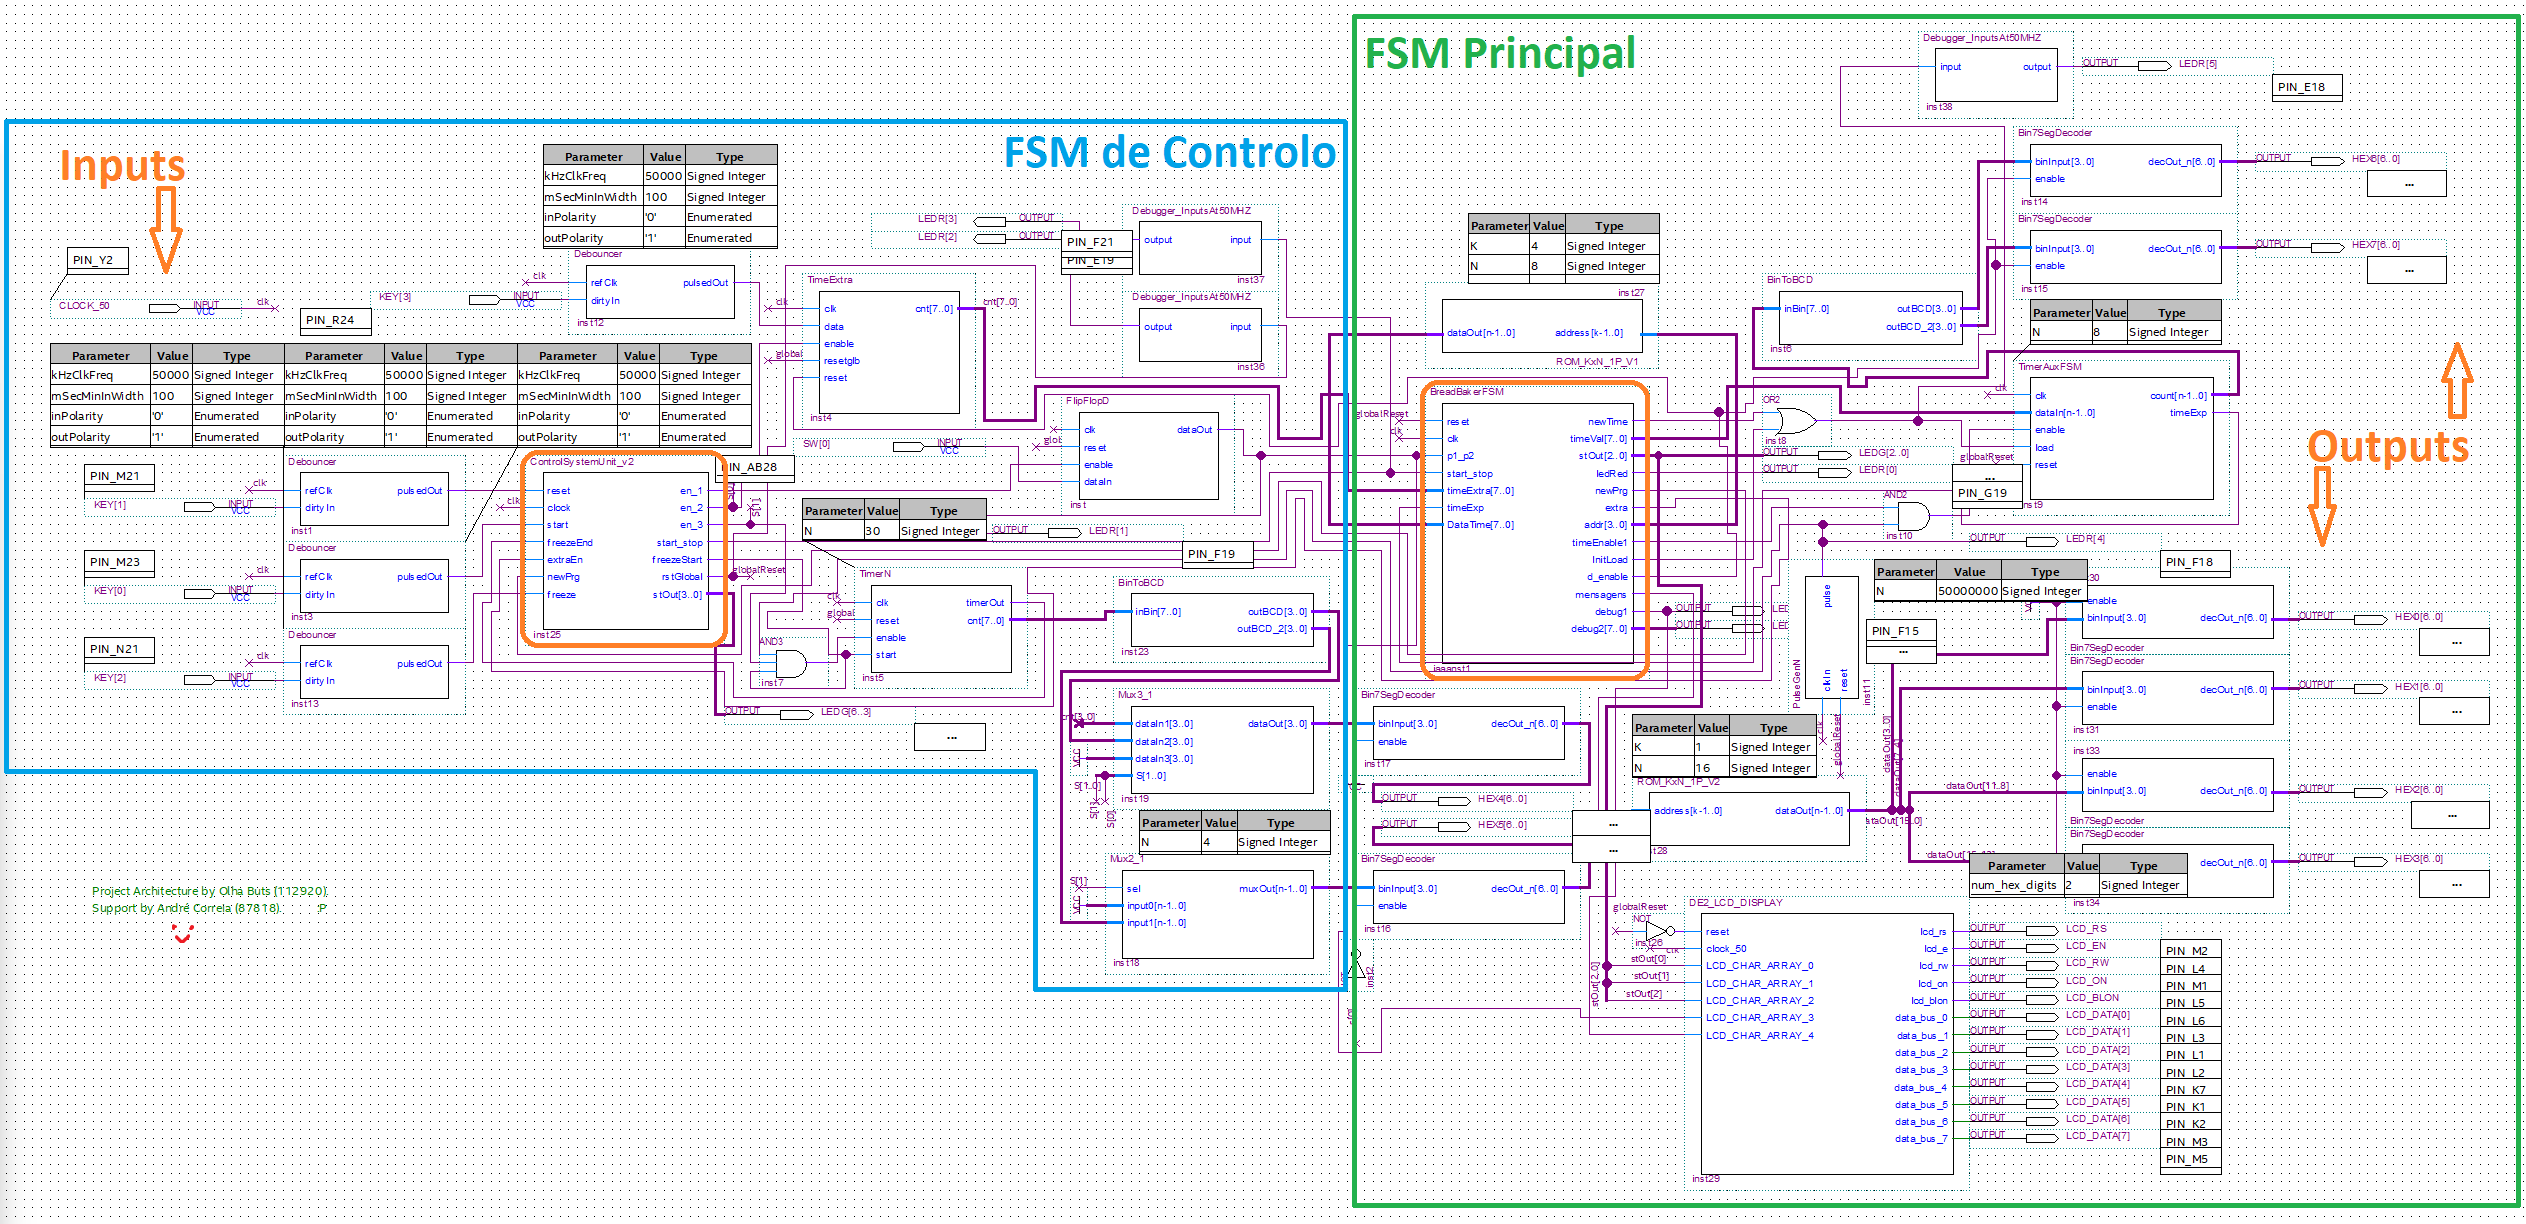
\includegraphics[width=335pt]{images/fase2v9_2}
	\caption{Diagrama Lógico do Sistema.}
	\label{fig:imagem1}
\end{figure}
\\
Assim, simplifica-se o circuito lógico através da abstração representada pela Figura 2.2 onde se destaca, conceptualmente, o sistema. Nesta Figura pode-se identificar que o sistema é constituído por duas FSM principais que controlam logicamente o conjunto de \textit{inputs} e \textit{outputs} fornecidos pela FPGA. A FSM de Controlo pode ser descrita pela responsabilidade dos mecanismos de \textit{start}/\textit{stop}, \textit{reset}, temporizadores (ligados à lógica de adição de tempos extra no início, ou no final), e pela seleção do modo de programa (tipo de pão Caseiro, ou Rústico). A FSM Principal é reponsável por toda a \textit{pipeline} de 'fazer pão' -- isto é, os estados de amassar, levedar e cozer.
\begin{figure}[h!] % Este [h!] força a imagem a aparecer onde é chamada.
	\center
	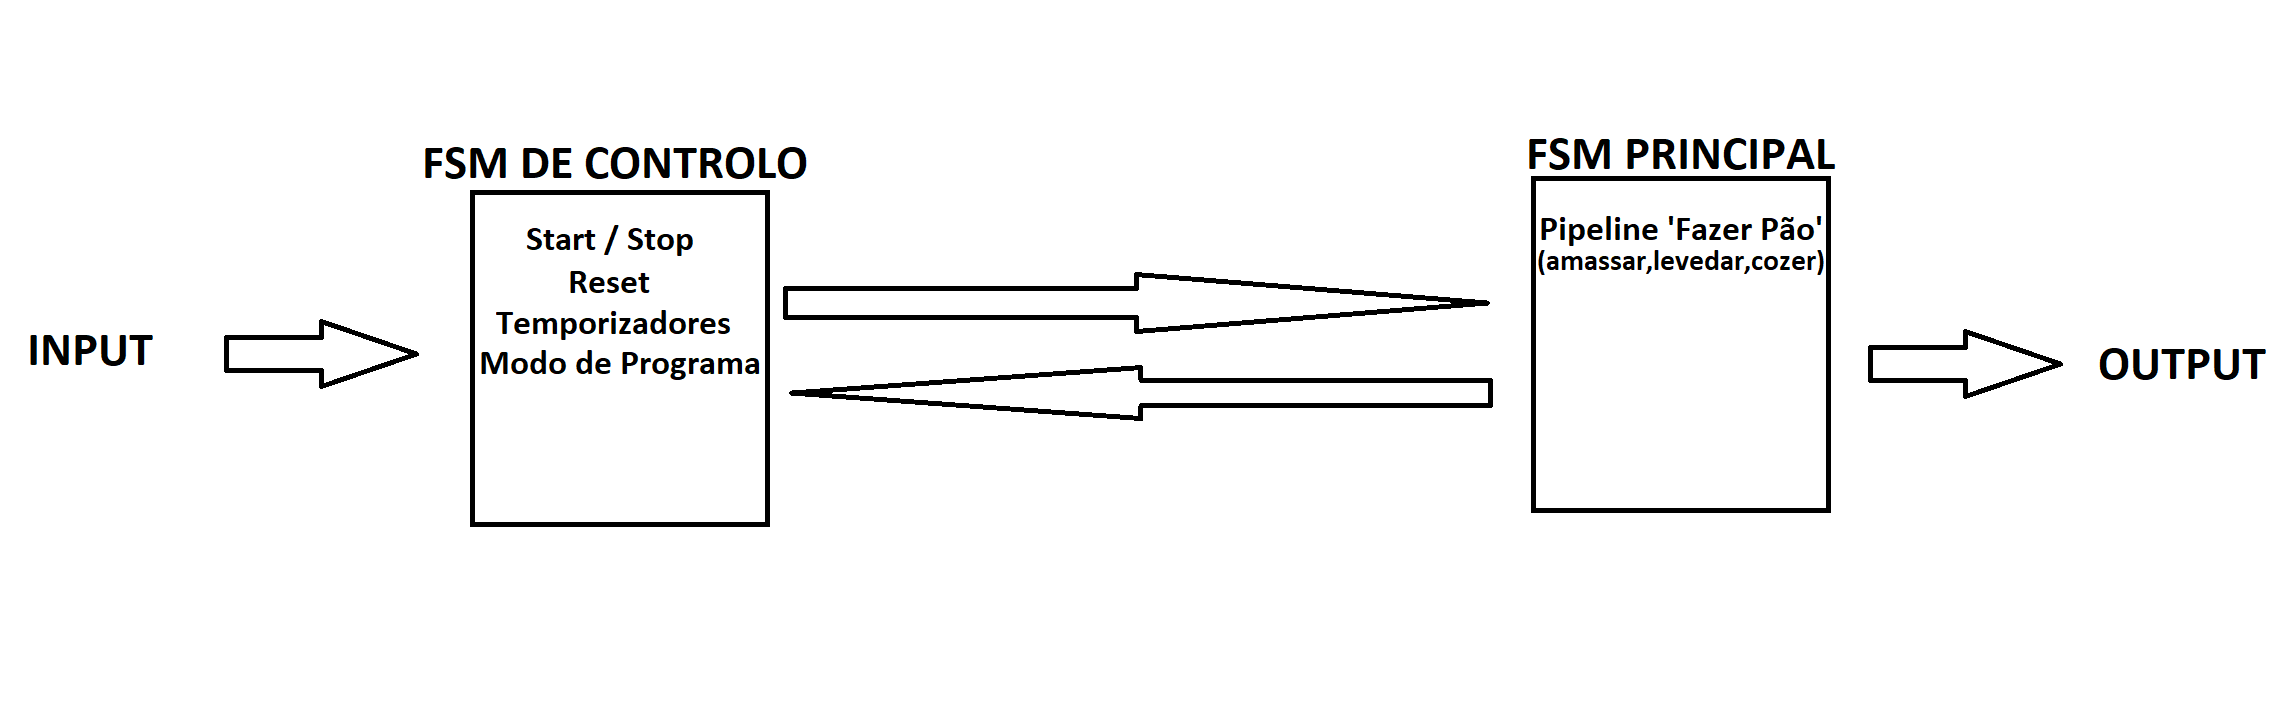
\includegraphics[width=250pt]{images/SistemaAbstrato_2}
	\caption{Abstração do Diagrama Lógico do Sistema.}
	\label{fig:imagem2}
\end{figure}

\section{Implementação do Sistema}
Nesta secção ilustram-se alguns aspetos da implementação da arquitetura anteriormente apresentada, tais como os diagramas de estados das FSM de Controlo e FSM Principal.
\\\\
Deste modo, começa-se por analisar o diagrama de estados da FSM de Controlo (ver Figura 2.3) onde se destaca a responsabilidade de iniciar a \textit{pipeline} da FSM Principal, assim como a responsabilidade de pausar todo o procedimento -- seja no momento de amassar, levedar, ou amassar o pão. Além disto, a Figura 2.3 demonstra o controlo dos tempos extras (inicial, ou final).
\begin{figure}[h!] % Este [h!] força a imagem a aparecer onde é chamada.
	\center
	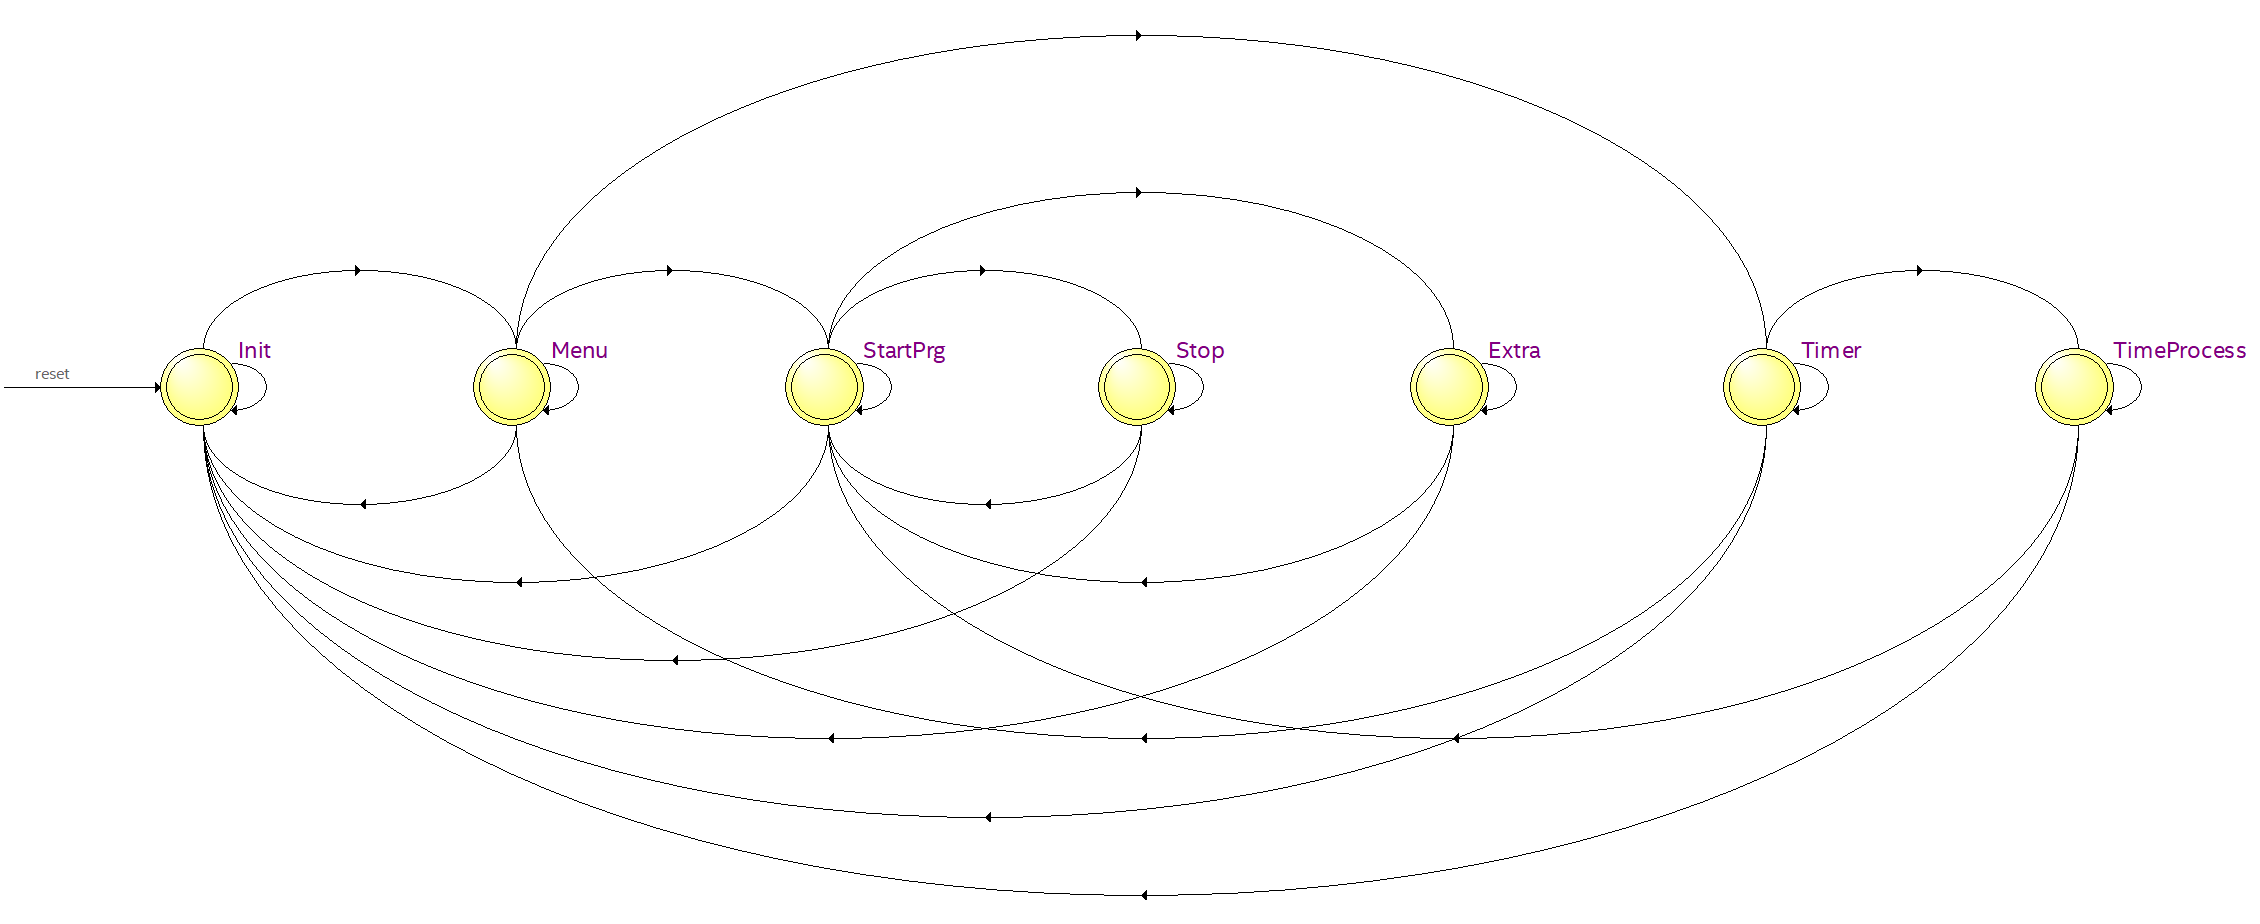
\includegraphics[width=350pt]{images/FSM1_2}
	\caption{Diagrama de Estados da FSM de Controlo.}
	\label{fig:imagem3}
\end{figure}
\\
O conjunto de lógica que suporta esta FSM é constituído por entradas (\textit{keys} e \textit{switches}), por \textit{debouncers}, por \textit{Flip-Flops} e pelos temporizadores responsáveis pelos tempos extra inicial e final (ver a abstração apresentada na Figura 2.4).
\begin{figure}[h!] % Este [h!] força a imagem a aparecer onde é chamada.
	\center
	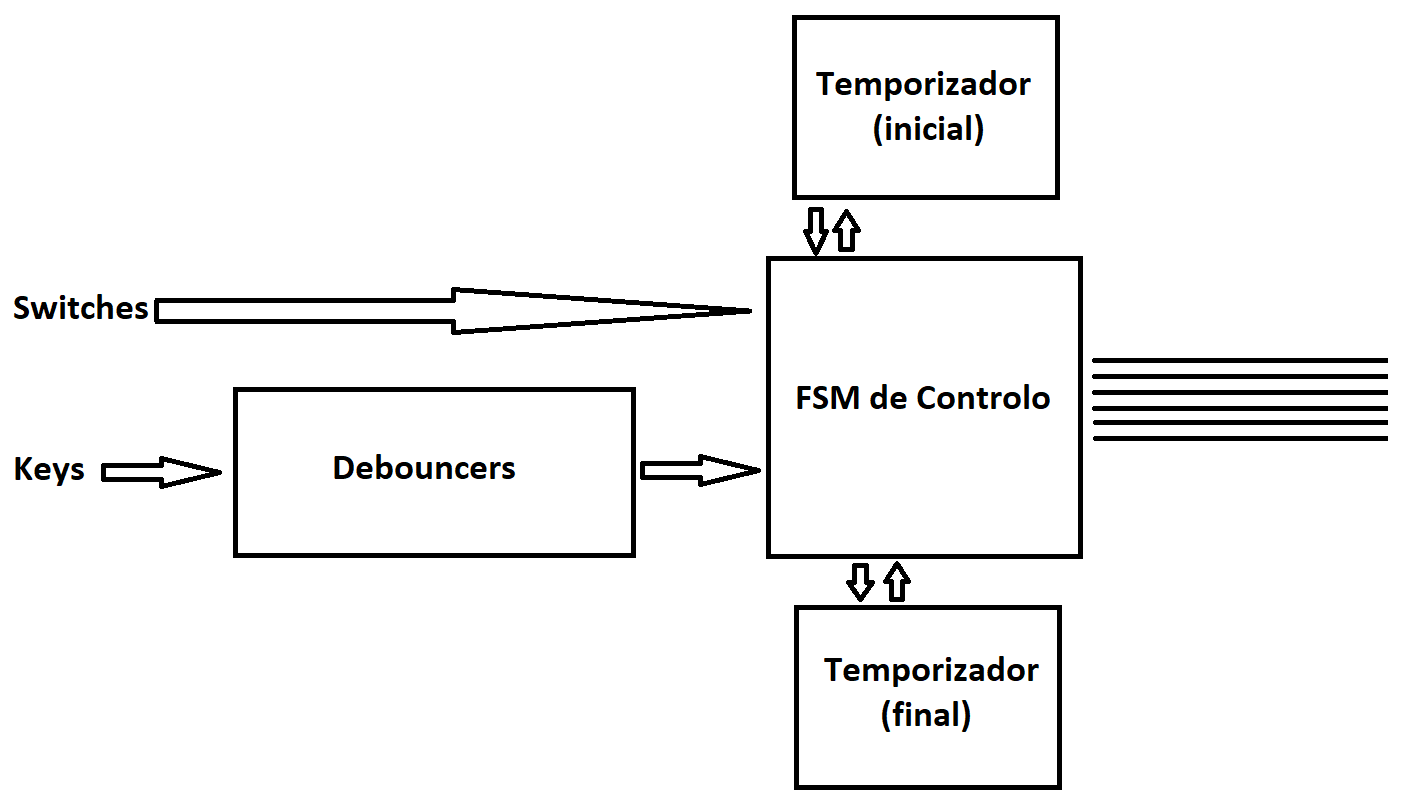
\includegraphics[width=250pt]{images/FSM1_Abstracao}
	\caption{Abstração da Zona da FSM de Controlo.}
	\label{fig:imagem4}
\end{figure}
\\\\
Relativamente à FSM Principal, apesar desta conter uma interface que alimenta alguns sinais de input da FSM de Controlo (por exemplo, o sinal "\textit{newPrg}" que indica que terminou o seu ciclo), denota-se uma responsabilidade quase total pela pipeline de amassar, levedar, e cozer o pão (ver Figura 2.5) -- onde a diferença entre o pão caseiro e rústico é no tempo de amassar (10s/15s, respetivamente) e de levedar (04s/08s); cozer (10s/10s) -- sendo que os tempos específicos para cada etapa são alimentados por uma \textit{\textbf{R}ead \textbf{O}nly \textbf{M}emory} (ROM).
\begin{figure}[h!] % Este [h!] força a imagem a aparecer onde é chamada.
	\center
	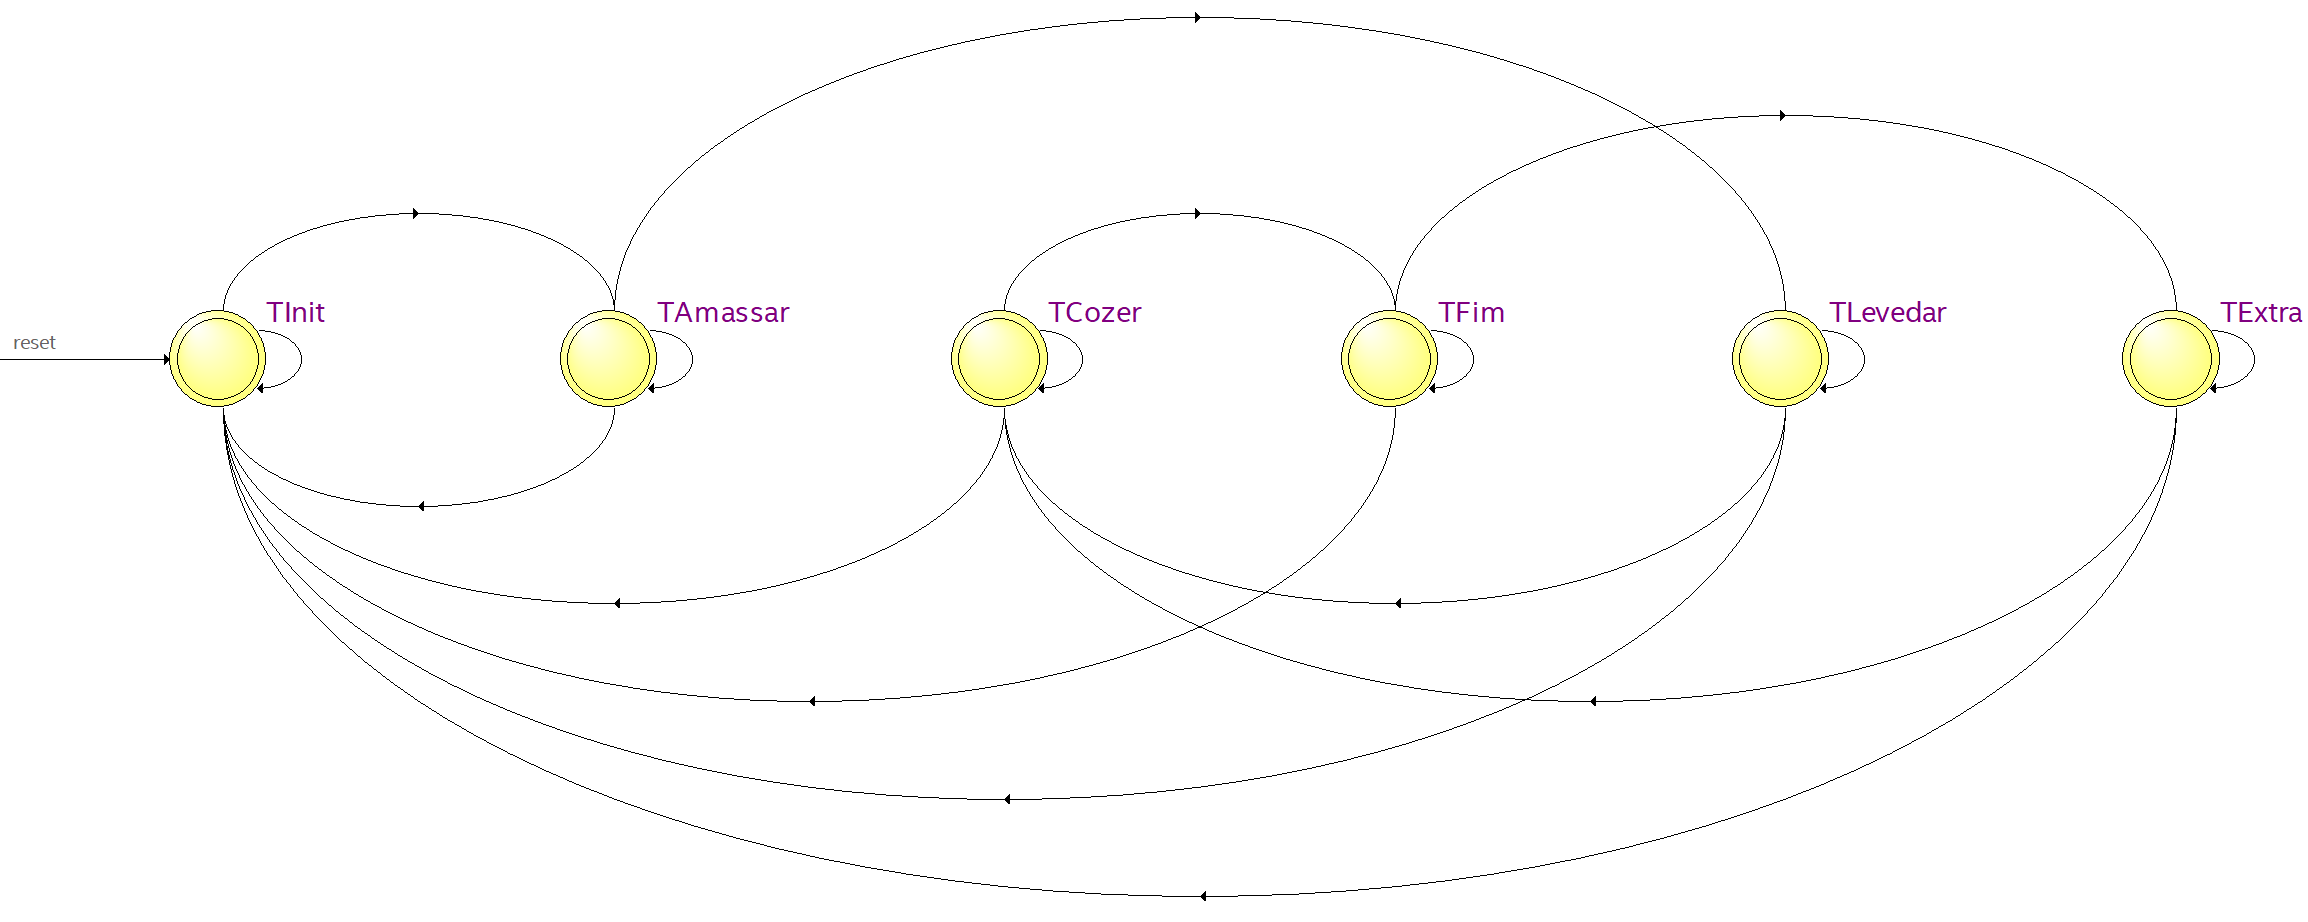
\includegraphics[width=350pt]{images/FSM2_2}
	\caption{Diagrama de Estados da FSM Principal.}
	\label{fig:imagem5}
\end{figure}
\\
Os dispositivos lógicos que constituem esta zona da responsabilidade da FSM Principal são (entre outros): descodificadores de binário para \textbf{B}inary-\textbf{C}oded \textbf{D}ecimal (BCD), descodificadores de binário para \textit{7-Segment}, ROMs, e contadores (ver a abstração apresentada na Figura 2.6).
\begin{figure}[h!] % Este [h!] força a imagem a aparecer onde é chamada.
	\center
	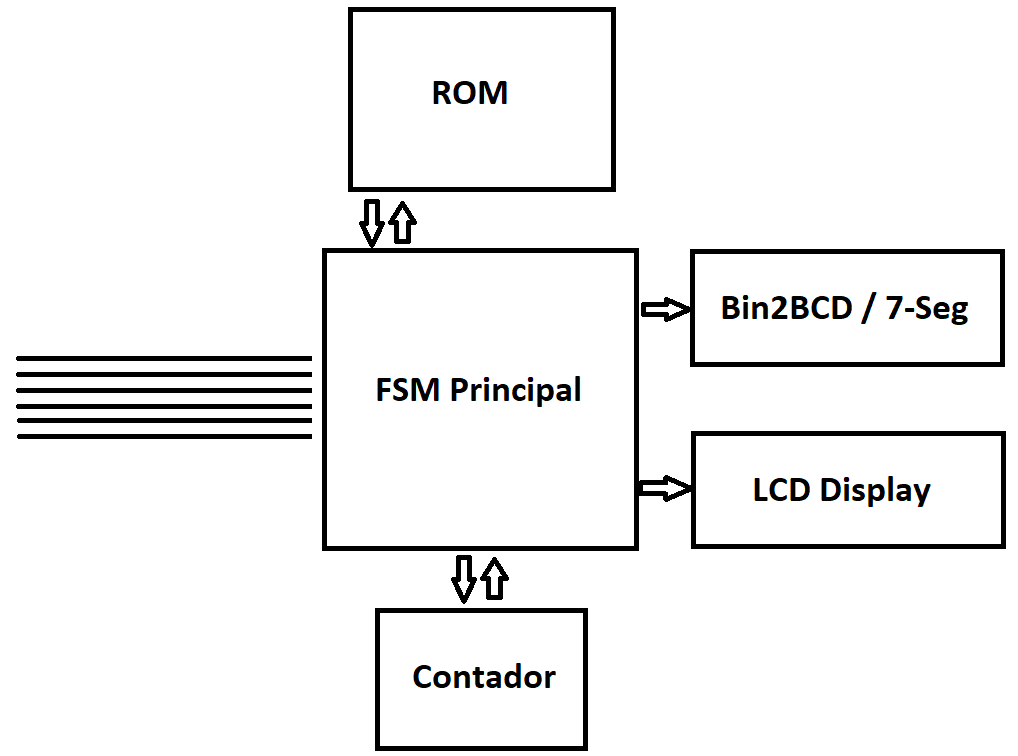
\includegraphics[width=200pt]{images/FSM2_Abstracao}
	\caption{Abstração da Zona da FSM Principal.}
	\label{fig:imagem6}
\end{figure}
\\
Contudo, o sistema contém outra lógica de suporte fulcral que não está mencionada em nenhuma das duas abstrações anteriormente apresentadas, tal como geradores de pulsos.

\section{Validação do Sistema}
Esta última secção do Desenvolvimento do Sistema Digital (Capítulo 2) tem como objetivo abordar os procedimentos implementados para validação do sistema -- com foco sobre a validação das FSM usando \textit{testbenches} desenhadas em VHDL. Contudo, também se aplicou uma rotina de interação com a máquina na ótica do utilizador (num formato de desenvolvimento em FPGA) em cada nova versão da implementação.
\\
Neste sentido, verifica-se na Figura 2.7 a correta transição de estados da FSM de Controlo quando aplicados diferentes valores nos seus inputs. É de se notar que esta FSM de Controlo tem como principais blocos lógicos \textit{standard} dois temporizadores (que são responsáveis pelo tempo extra no inicio, ou no final), assim como um sinal proveniente da FSM Principal (que indica se o ciclo da \textit{pipeline} terminou). Deste modo, a manipulação destes valores de acordo com comportamentos esperados -- e outros aleatórios (\textit{edge-cases} potencialmente problemáticos) -- permite validar o bloco lógico como corretamente funcional.
\begin{figure}[h!] % Este [h!] força a imagem a aparecer onde é chamada.
	\center
	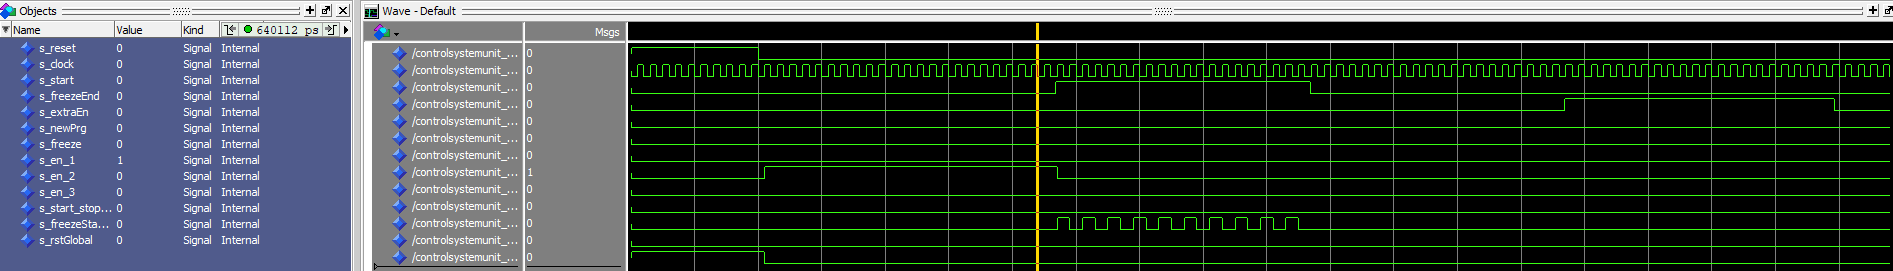
\includegraphics[width=335pt]{images/FSM1_TB_2}
	\caption{Testbench da FSM de Controlo.}
	\label{fig:imagem7}
\end{figure}
\\
Relativamente à FSM Principal, como se verifica na Figura 2.8, aplicando a mesma metodologia de manipulação das entradas, obtem-se o comportamento esperado (correto) do bloco lógico.
\begin{figure}[h!] % Este [h!] força a imagem a aparecer onde é chamada.
	\center
	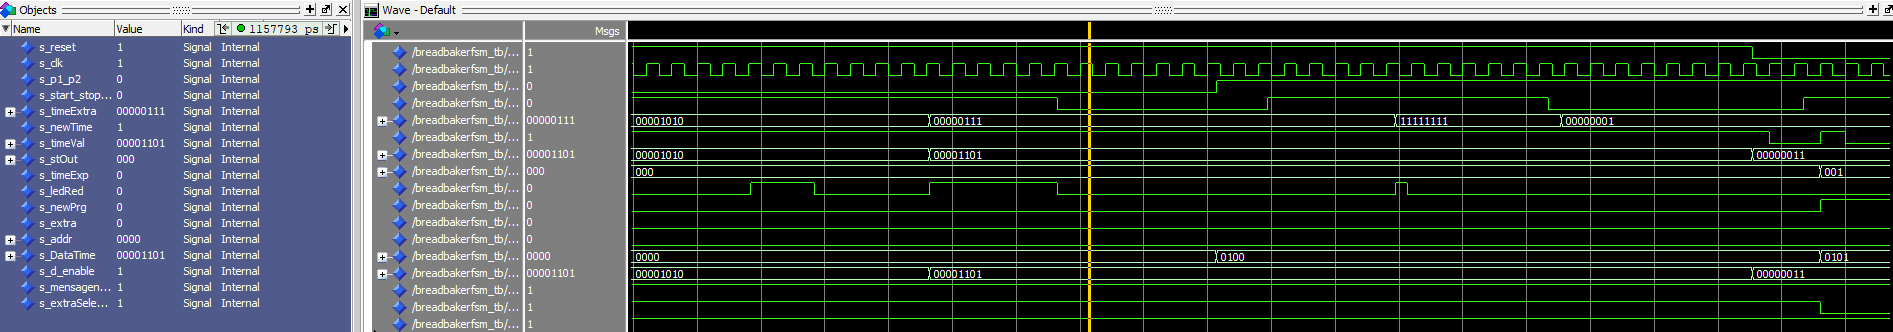
\includegraphics[width=335pt]{images/FSM2_TB_3}
	\caption{Testbench da FSM Principal.}
	\label{fig:imagem8}
\end{figure}
\\
Por fim, indica-se a Figura 2.9 que demonstra o teste efetuado ao sistema como um todo (\textit{Top-Level}). Nesta Figura, verifica-se o correto comportamento da Máquina Automática de Fazer Pão -- exatamente como analisado manualmente na FPGA.
\begin{figure}[h!] % Este [h!] força a imagem a aparecer onde é chamada.
	\center
	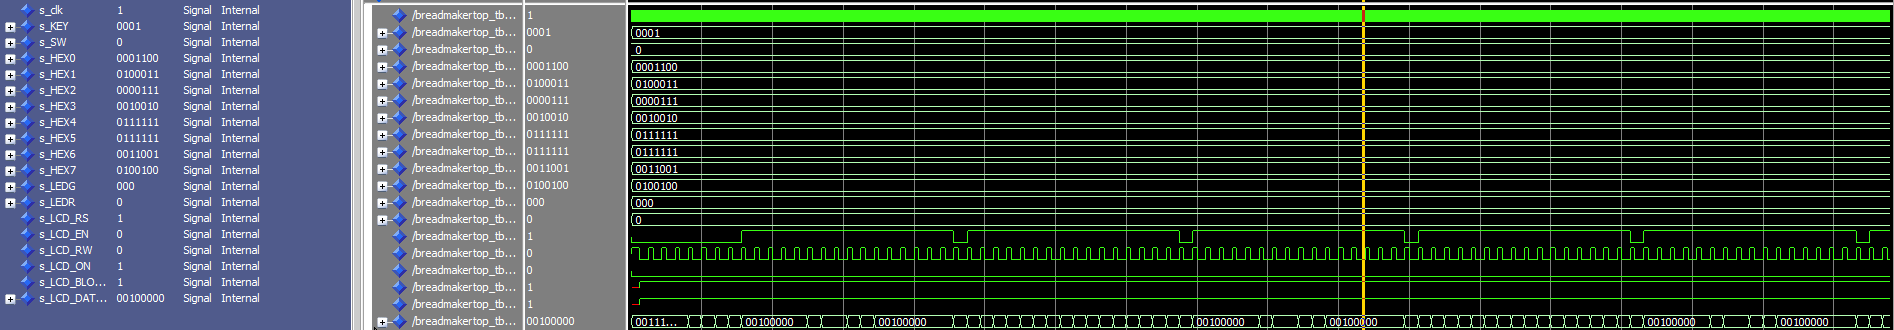
\includegraphics[width=335pt]{images/TopLevelTB_2}
	\caption{Testbench do Top-Level do Sistema.}
	\label{fig:imagem9}
\end{figure}

\chapter{Manual de Utilizador}
\label{chap.manualUtilizador}
Tomando os passos de preparação da FPGA como garantidos -- connectar (USB e \textit{Power Delivery}), e submeter o projeto para a FPGA -- então o utilizador, após ligar o dispositivo, é recebido por um menu de utilizador.
\begin{itemize}
	\item SW[0] - Permite alterar o modo de operação (entre Pão Caseiro e Pão Rústico).
	\item KEY[0] - Inicia o processo de 'fazer pão' (\textit{start}).
	\item KEY[2] - Permite adicionar um tempo extra de atraso ao iniciar do processo de 'fazer pão' (necessário depois premir KEY[0] para iniciar).
\end{itemize}
Depois de iniciar o processo de 'fazer pão', o utilizador pode pausar esta \textit{pipeline} em qualquer etapa do processo, premindo o KEY[0] (\textit{stop}).
\\\\
Com isto, no final deste processo de 'fazer pão', o utilizador é recebido por uma mensagem que permite adicionar um tempo extra de cozedura. Para isto, terá de premir o KEY[3] para incrementar o temporizador (que tem um alcance limitado e cíclico), sendo necessário premir o KEY[0] (\textit{start/stop}) para iniciar este processo de aquecimento extra.
\\\\
É de se notar que, sempre que a máquina acaba a sua \textit{pipeline}, o utilizador tem a opção de um aquecimento extra (quantas vezes assim pretender) -- sendo que para quebrar este ciclo, o utilizador tem de ter o temporizador a 0 e premir o KEY[0] (\textit{start/stop}).
\\\\
Por fim, o utilizador em qualquer momento pode fazer um \textit{reset} à maquina premindo o KEY[1]. Esta ação irá levar a máquina para o estado do menu (inicial) de utilizador.


\chapter{Conclusões}
\label{chap.conclusao}
A arquitetura da Máquina Automática de Fazer Pão e a posterior implementação através de Máquinas de Estados Finitos Comunicantes, e toda a envolvente lógica digital, demonstrou atingir um nível de complexidade que necessita de procedimentos de desenvolvimento bem definidos desde o início do projeto.
\\\\
Deste modo, é de importância realçar a necessidade de estratégias de desenvolvimento faseadas e de mecanismos de controlo, tais como versões de projeto, assim como metodologia em todas as etapas do projeto. Por se prever este nível de complexidade, esta equipa preparou um repositório na plataforma GitHub onde se encontram múltiplas versões do Projeto, documentação de suporte ao desenvolvimento, versões do presente relatório, e outro material usado (como \textit{drivers} do LCD).
\\\\
Além disto, canais de comunicação bem definidos, assim como o estabelecimento de um líder para cada componente do Projeto Final são condições necessárias, e aplicadas neste projeto, para ver o produto final com sucesso e a qualidade esperada pela equipa. Deste modo, destaca-se a \textit{Lead-Architect} Olha Buts que tomou controlo da arquitetura e implementação do sistema digital.
\\\\
Em suma, este projeto decorreu como esperado. Com isto, o nível de dificuldade superou ligeiramente as expectativas iniciais, mas toda a preparação prévia de organização do trabalho da equipa (parágrafos anteriormente mencionados) foi fulcral para ver este projeto sucedido. Portanto, o Projeto Final de LSD é sem dúvida um elemento de avaliação necessário para garantir a consolidação dos conhecimentos lecionados nesta UC, mas também para garantir que os alunos têm mecanismos de trabalho em equipa e uma ótica orientada aos objetivos.
\\\\
Assim, a percentagem de trabalho é:
\begin{itemize}
	\item \textbf{50\%}: Olha Buts (112920) - o.buts@ua.pt
	\item \textbf{50\%}: André Correia (87818) - amcorreia@ua.pt
\end{itemize}


%\textbf{Repositório GitHub:} labi2023gN

%%%%%%%%%%%%%%%%%%%%%%%%%%%%%%%%%
%\chapter*{Acrónimos}
%\begin{acronym}
%\acro{ua}[UA]{Universidade de Aveiro}
%\acro{leci}[LECI]{Licenciatura em Engenharia de Computadores e Informática}
%\acro{glisc}[GLISC]{Grey Literature International Steering Committee}
%\acro{lsd}[LSD]{Laboratório de Sistemas Digitais}
%\acro{vhdl}[VHDL]{Very \textit{High Speed Integrated Circuits} Hardware Description Language}
%\end{acronym}


%%%%%%%%%%%%%%%%%%%%%%%%%%%%%%%%%
\printbibliography

\end{document}
